% Formatage général
	\documentclass[a4paper,11pt]{article}
	\usepackage{lmodern}
	\usepackage[T1]{fontenc} % Encodage des caractères spéciaux
	\usepackage{helvet} % Police équivalent Arial
	\usepackage[french]{babel} % Localisation en français
	\frenchbsetup{StandardLists=true} % Pour dire à babel de garder le formatage standard (anglais) des listes à puce
	\usepackage{csquotes} % Pour remplacer automatiquement les guillemets par des guillemets typographique
	\MakeOuterQuote{"} % Le caractère utilisé pour rentrer les guillemets dans le code est le "
	
% Dimensions
	\usepackage[margin=2cm]{geometry} % Marges
	\setlength{\headheight}{30pt}
	\addtolength{\topmargin}{-18pt}
	\setlength{\parindent}{0pt} % Largeur de l'alinéa

% Couleurs
	\usepackage{xcolor} % Permet de passer un texte en couleur avec la commande \textcolor{color}{text}
	\definecolor{parissaclay}{HTML}{63003C} % Prune officiel de l’Université Paris-Saclay
	\definecolor{gamboge}{rgb}{0.89, 0.61, 0.06} % Couleur perso orange appliquée aux subsubsections
	
% Formatage des titres
	\usepackage{titlesec} % Package utilisé pour formater les titres
	\setcounter{secnumdepth}{3} % Numéortation jusqu'au niveau subsubsection
	
	\titleformat{\section} % Formatage des sections
		{\fontsize{18}{18}\bfseries\color{parissaclay}} % Titre en 18 pt, gras, couleur Paris-Saclay
		{\Roman{section}.} % Numérotation romaine majuscule suivie d'un point
		{1ex} % Un espace entre le numéro et le titre
		{}
	
	\titleformat{\subsection} % Formatage des sous-sections
		{\fontsize{16}{16}\bfseries\color{parissaclay}} % Titre en 16 pt, gras, couleur Paris-Saclay
		{\Alph{subsection}.} % Numérotation en lettre majuscule suivie d'un point
		{1ex} % Un espace entre le numéro et le titre
		{}
	
	\titleformat{\subsubsection} % Formatage des sous-sous-sections
		{\fontsize{15}{15}\bfseries\color{gamboge}} % Titre en 15 pt, gras, couleur orange
		{(\alph{subsubsection})} % Numérotation en lettre minuscule entourée de parenthèses
		{1ex} % Un espace entre le numéro et le titre
		{}
	
% En-tête et pied de page
	\usepackage{fancyhdr} % Package utilisé pour personnaliser facilement en-tête et pied-de-page
	\renewcommand{\headrulewidth}{0pt} % Épaisseur de la ligne de séparation entre en-tête et corps du rapport
	
	\fancypagestyle{main}{\fancyhf{} % En-tête et pied de page pour toutes les autres pages
		\fancyhead[L]{
\includegraphics[width=2cm]{images/paris-saclay.png}} % En haut à gauche, le logo Paris-Saclay
		\fancyhead[R]{Master SETI 2026-2027} % En haut à droite, la formation et l’année
		\fancyfoot[C]{\thepage} % En bas au centre, le numéro de page
	}
	\pagestyle{main}
		
% Page de titre
	\newcommand{\HRule}[1]{\rule{\linewidth}{#1}} % Ligne de séparation horizontale d'une épaisseur donnée

% Figures
	\usepackage{graphicx} % Permet l'ajout d'images en spécifiant la taille
	\usepackage{subcaption} % Package utilisé pour avoir des sous-figures avec chacune une légende
	\usepackage[labelfont=bf]{caption} % "Figure" et numéro en gras
	
\usepackage{amsmath}
\usepackage{booktabs,tabularx,float}

% Liens
	\usepackage[colorlinks=true,linkcolor=black,urlcolor=parissaclay]{hyperref}

\begin{document}
	
	\title{
		\begin{figure}[htb]
			\begin{minipage}[t]{.45\textwidth}
				\centering
				
\includegraphics[width=6cm]{images/paris-saclay.png}
			\end{minipage}
			\hfill
			\begin{minipage}[t]{.45\textwidth}
				\centering
				\raggedleft\Large{\textbf{Master SETI}\\ 2026-2027}
			\end{minipage}  
		\end{figure}
		\vspace{2cm}
		\HRule{1.5pt} \\ [0.5cm]
		\LARGE \textbf{\Large{RAPPORT DE TP}\\ [5mm]
		\huge{\textcolor{parissaclay}{TP 1 : Calcul de racine carrée}}}
		\HRule{1.5pt} \\ [3mm]
		
		\normalsize
		\vspace{1cm}
		\vfill
	}
	
	\author{
		Côme CERVANTES \and Joseph MOUSCADET
	}
	
	\date{
		Nous attestons que ce travail est original,\\
		qu’il est le fruit d’un travail commun au binôme et qu’il a été rédigé de manière autonome.\\ [2mm]
		\textbf{Paris, le 07/10/2026}
	}
	
	\maketitle % Page de titre
\clearpage
\pagestyle{main}
\section{Architecture séquentielle comportementale}
\subsection{Principe et graphe d’état}
\textbf{Question a).} Nous cherchons à calculer la racine carrée entière d’un nombre non signé $A$ codé sur $2n$ bits, avec un résultat sur $n$ bits. La description doit être synthétisable, utiliser un seul processus et réaliser chacune des $n$ itérations en un cycle. Le résultat attendu est $Z=\lfloor\sqrt{A}\rfloor$, ce qui se vérifie par $Z^2\leq A<(Z+1)^2$.

\begin{figure}[H]
    \centering
    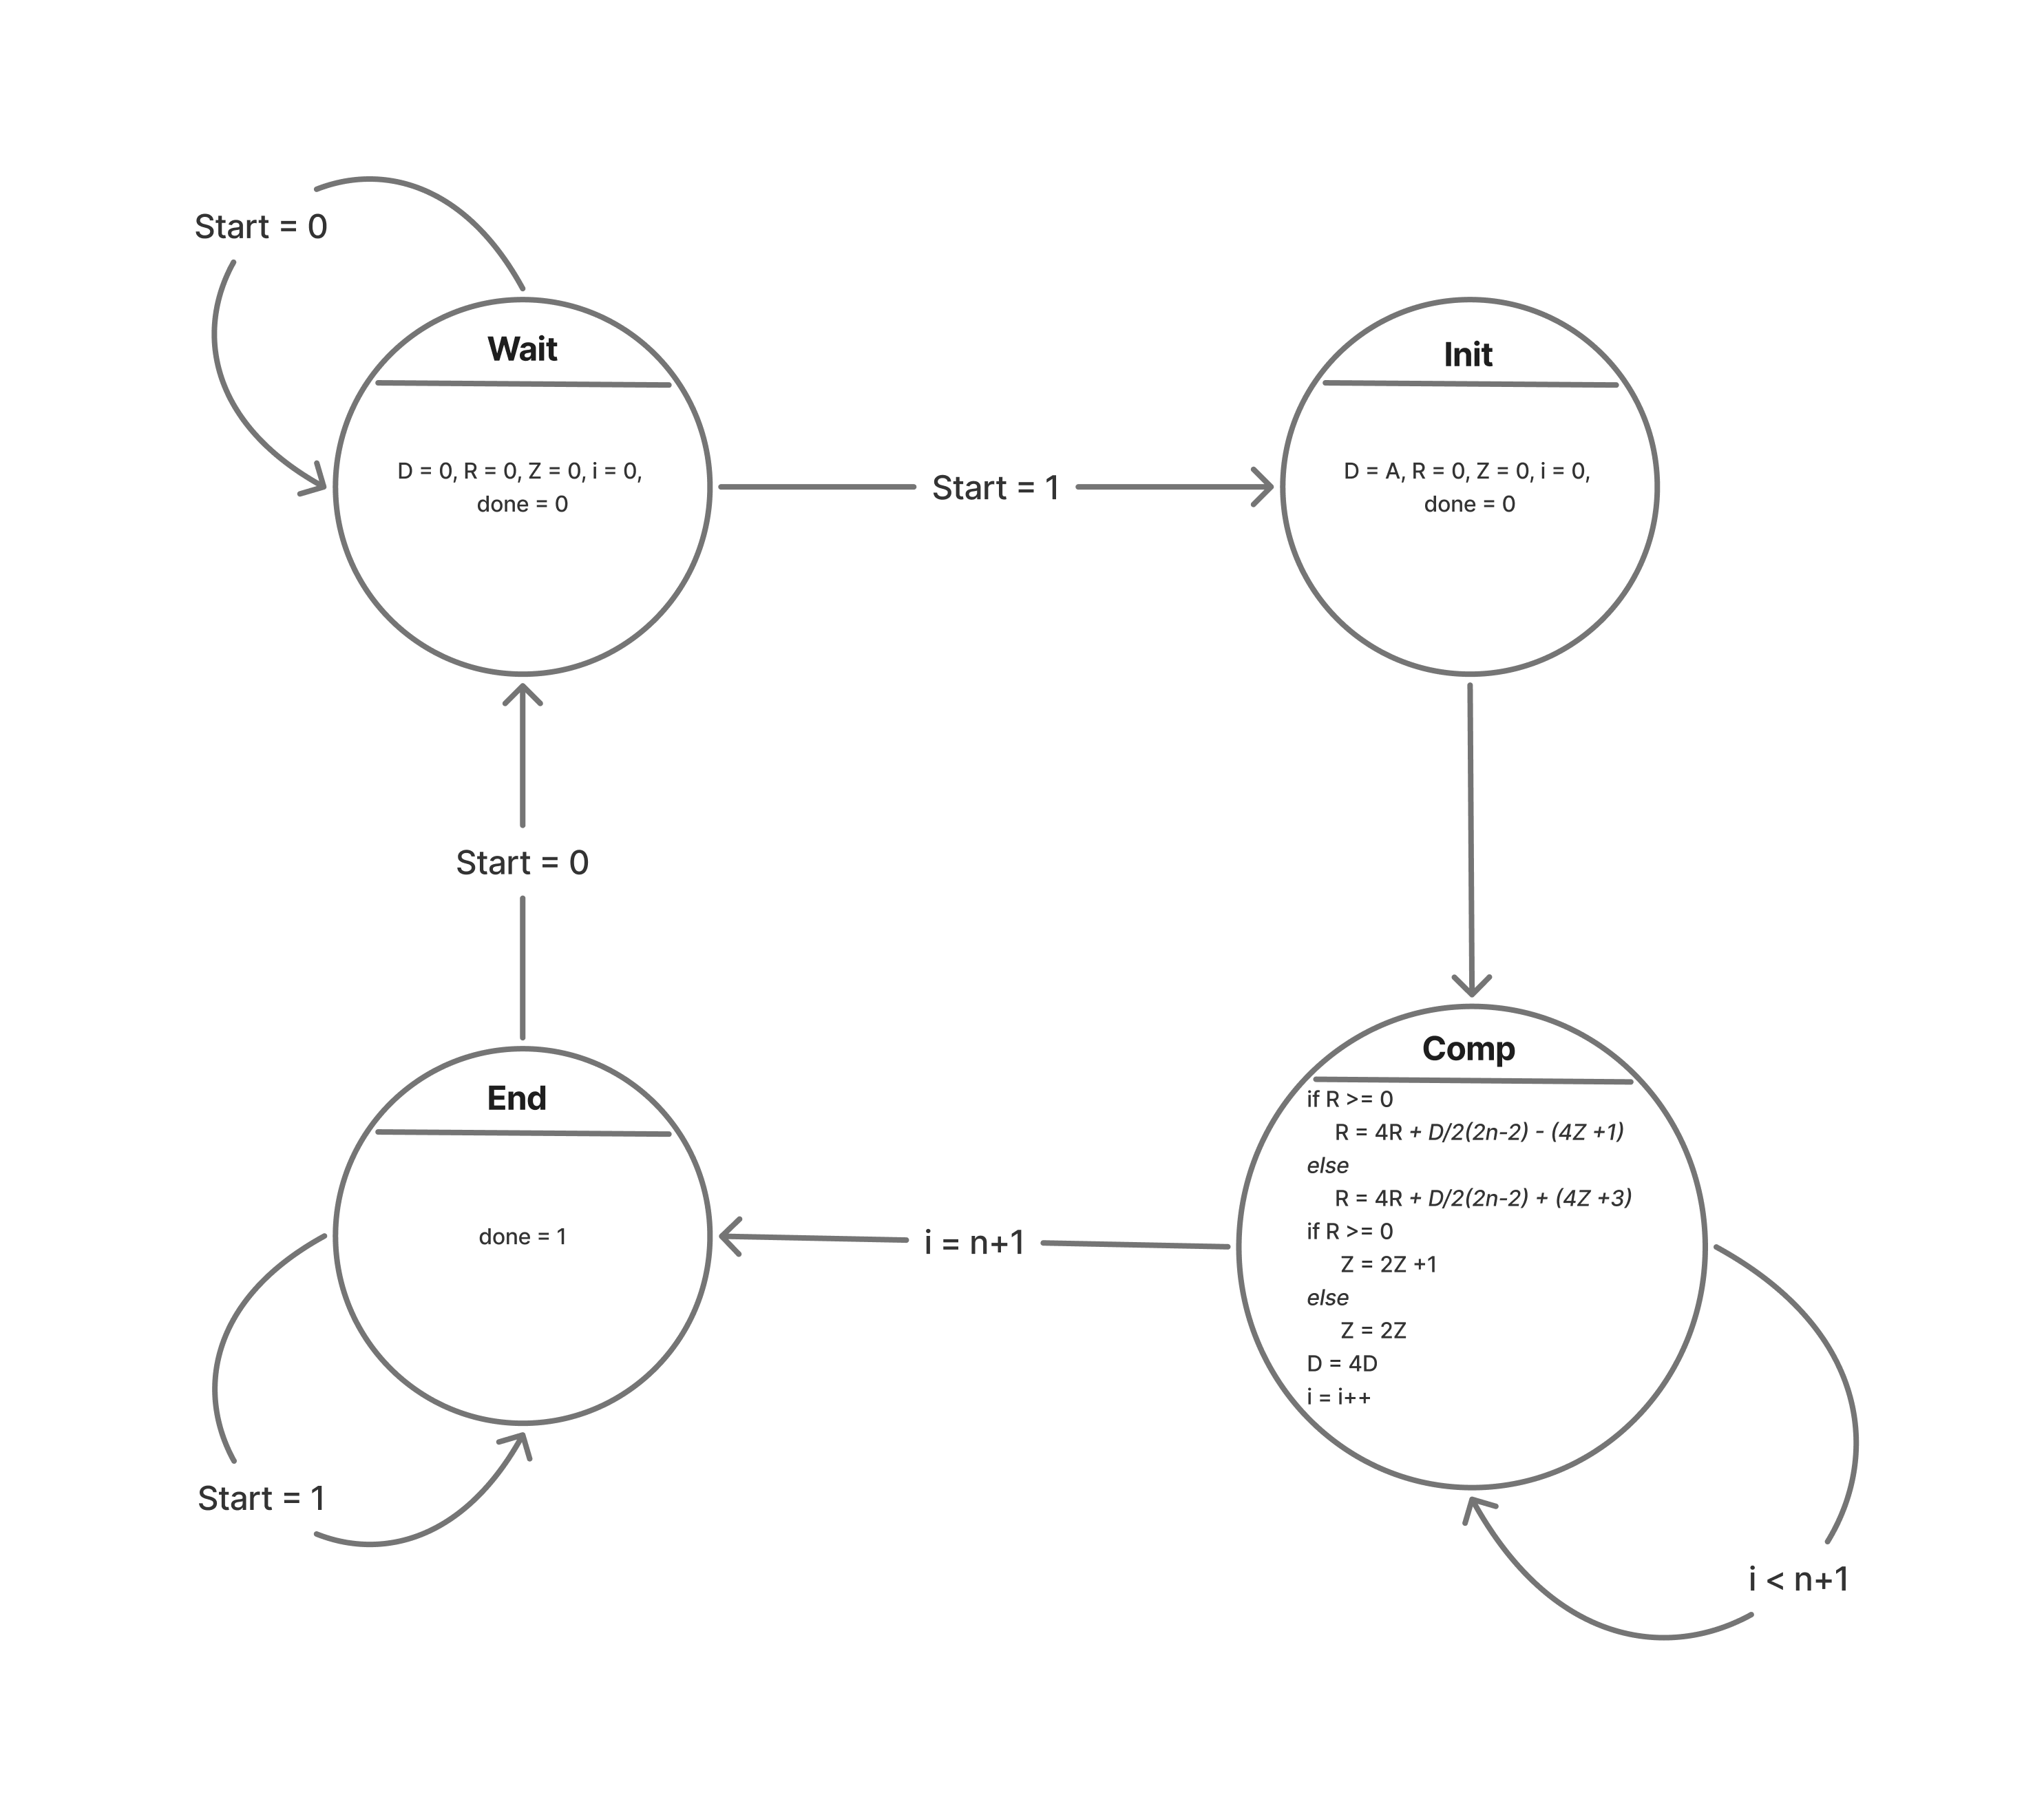
\includegraphics[width=.83\linewidth,height=11.3cm,keepaspectratio]{images/graphe_detat.png}
    \caption{Graphe d’état utilisé pour organiser l’architecture séquentielle.}
    \label{fig:etats}
\end{figure}

Le graphe de la figure~\ref{fig:etats} sépare l’attente, le chargement, le calcul et la fin du traitement. Il correspond aux quatre états du type énuméré utilisé dans \texttt{sqrt\_seq.vhd} :
\begin{itemize}
    \item \texttt{wait\_state} : mise à zéro de $D$, $R$, $Z$, du compteur et de \texttt{done}. Le circuit attend \texttt{start = '1'} pour passer à l’initialisation.
    \item \texttt{init\_state} : chargement de $A$ dans $D$, remise à zéro des autres données, puis passage au calcul au cycle suivant.
    \item \texttt{comp\_state} : exécution d’une itération par front montant. L’état est conservé tant que $i<n-1$ ; la dernière itération conduit à \texttt{end\_state}.
    \item \texttt{end\_state} : \texttt{done} passe à 1. Le résultat est conservé ; le circuit reste dans cet état si \texttt{start = '1'}, sinon il retourne à l’attente.
\end{itemize}
Le reset actif à 1 impose l’état d’attente de manière asynchrone. Sur le dessin, le terme de division doit se lire $D/2^{2n-2}$ et l’incrément du compteur $i\leftarrow i+1$ ; les étiquettes $i=n+1$ et $i<n+1$ doivent être corrigées en $i=n-1$ et $i<n-1$ pour correspondre au compteur du code.

\clearpage
\pagestyle{main}
\subsection{Algorithme et choix des types}
L’algorithme construit la racine bit par bit, en traitant les bits de $A$ par paires, depuis les poids forts. Au début d’une itération, on extrait $p=D(2n-1\ \mathrm{downto}\ 2n-2)$, soit un entier entre 0 et 3. Avec les anciennes valeurs de $R$ et $Z$, on calcule :
\[
R_{\mathrm{nouveau}}=
\begin{cases}
4R+p-(4Z+1), & R\geq 0,\\
4R+p+(4Z+3), & R<0.
\end{cases}
\]
Le signe du \emph{nouveau} reste détermine ensuite le bit ajouté à la racine :
\[
Z_{\mathrm{nouveau}}=
\begin{cases}
2Z+1, & R_{\mathrm{nouveau}}\geq 0,\\
2Z, & R_{\mathrm{nouveau}}<0.
\end{cases}
\qquad D_{\mathrm{nouveau}}=(4D)\bmod 2^{2n}.
\]
Les multiplications par 2 et par 4 sont réalisées par des décalages à gauche de un ou deux bits. L’extraction des deux bits de poids fort remplace la division entière par $2^{2n-2}$. Le décalage de $D$ élimine la paire déjà traitée et présente la suivante. Il n’est donc pas nécessaire d’utiliser un diviseur ou un multiplicateur général.

\begin{table}[H]
\centering
\small
\renewcommand{\arraystretch}{1.22}
\begin{tabularx}{\linewidth}{@{}p{2.7cm}p{4.5cm}X@{}}
\toprule
\textbf{Élément} & \textbf{Type et taille pour $n=32$} & \textbf{Rôle et justification}\\
\midrule
\texttt{clk, rst, start, done} & \texttt{std\_logic}, 1 bit & Signaux de commande et indication de fin.\\
\texttt{A} & \texttt{std\_logic\_vector}, 64 bits & Bus d’entrée ; converti en \texttt{unsigned} lors du chargement.\\
\texttt{Result} & \texttt{std\_logic\_vector}, 32 bits & Bus de sortie, relié à $Z$ par une conversion de type.\\
$D$ (signal) & \texttt{unsigned}, $2n=64$ bits & Copie décalée de l’opérande, toujours non signée.\\
$Z$ (signal) & \texttt{unsigned}, $n=32$ bits & Racine partielle puis résultat entier non négatif.\\
$R$ (variable) & \texttt{signed}, $n+2=34$ bits & Reste partiel pouvant être négatif ; les bits supplémentaires servent au signe et aux opérations intermédiaires.\\
$i$ (signal) & \texttt{integer range 0 to n-1} & Compteur borné de 0 à 31, correspondant aux 32 itérations.\\
\texttt{curr\_state} & Type énuméré à quatre valeurs & Rend explicites les phases de commande de l’automate.\\
\bottomrule
\end{tabularx}
\caption{Signaux et variable de l’architecture comportementale.}
\label{tab:types}
\end{table}

Le paramètre générique $n$ fixe la largeur du résultat et le nombre d’itérations ; $n=32$ donne une entrée sur 64 bits. Le paquet \texttt{numeric\_std} fournit les opérations sur \texttt{signed} et \texttt{unsigned}. Les conversions et les appels à \texttt{resize} mettent les opérandes à la largeur de $R$ avant les additions, soustractions et décalages. Contrairement à la boucle décroissante du sujet, notre compteur est croissant : l’ordre des paires traitées reste identique, car il est imposé par le décalage de $D$.

\clearpage
\pagestyle{main}
\subsection{Un seul processus et une itération par cycle}
La commande et le calcul sont regroupés dans le processus \texttt{PCalc}, sensible à \texttt{clk} et \texttt{rst}. Hors reset, les mises à jour se font sur les fronts montants. L’affectation concurrente de \texttt{Result} à partir de $Z$ ne constitue pas un second processus de commande ; elle expose simplement le registre de résultat.

\medskip
\textbf{Pourquoi une variable pour $R$ ?} Une affectation de variable avec \texttt{:=} prend effet immédiatement dans l’exécution du processus. Le second test de signe utilise ainsi le reste qui vient d’être calculé au même front d’horloge. Une affectation de signal avec \texttt{<=}, suivie du même test dans ce processus, lirait encore l’ancienne valeur. Ce choix permet de respecter l’enchaînement de l’algorithme en un seul cycle par itération.

\medskip
La variable $R$ conserve néanmoins sa valeur entre deux activations du processus : elle représente ici une donnée mémorisée, et non une valeur automatiquement remise à zéro à chaque cycle. Les signaux $D$, $Z$ et $i$ sont également mémorisés, mais leurs nouvelles valeurs ne sont visibles qu’après l’exécution du processus. Les calculs du cycle utilisent donc l’ancien $Z$ et l’ancien $D$, conformément aux équations précédentes.

\medskip
\textbf{Interface de commande.} L’entrée $A$ doit être stable au front exécutant \texttt{init\_state}, où elle est effectivement copiée dans $D$. Elle n’est plus utilisée pendant les itérations. La sortie \texttt{Result} présente des valeurs partielles pendant le calcul ; elle doit être exploitée lorsque \texttt{done = '1'}. Maintenir \texttt{start} à 1 permet de conserver l’état de fin. Après sa remise à 0, l’automate retourne à l’attente, puis efface le résultat lors de l’exécution de cet état.

\subsection{Temps de calcul et organisation du testbench}
Le cœur du calcul réalise exactement $n$ itérations, donc $n$ cycles. Le protocole ajoute un cycle d’initialisation et un cycle pour exécuter l’état de fin et lever \texttt{done}. À partir du front qui détecte \texttt{start} dans l’état d’attente, les délais sont donc :
\[
N_{\mathrm{Result\ final}}=n+1,\qquad
N_{\mathrm{done}}=n+2,\qquad
t_{\mathrm{done}}=(n+2)T_{\mathrm{clk}}.
\]
Ces nombres désignent des \emph{intervalles} d’horloge depuis le front de détection. Depuis le chargement de $A$, \texttt{done} arrive après $n+1$ cycles. Le nombre d’itérations reste constant, quelle que soit la valeur de $A$.

\medskip
Dans \texttt{testbench.vhd}, $n=32$, le reset dure 5 ns et l’horloge a une période de 20 ns, soit 50 MHz en simulation. Le premier \texttt{start} est activé à 25 ns, détecté au front de 30 ns. Le déroulement déduit du code est :
\begin{table}[H]
\centering
\renewcommand{\arraystretch}{1.15}
\begin{tabular}{@{}ll@{}}
\toprule
\textbf{Événement du premier calcul} & \textbf{Instant}\\
\midrule
Détection de \texttt{start} & 30 ns\\
Chargement de $A=100$ dans \texttt{init\_state} & 50 ns\\
Première / dernière itération & 70 ns / 690 ns\\
Résultat final / activation de \texttt{done} & 690 ns / 710 ns\\
\bottomrule
\end{tabular}
\caption{Chronologie attendue d’après le testbench et l’automate.}
\end{table}
Le calcul itératif représente 640 ns ; le délai entre la détection de \texttt{start} et \texttt{done} vaut 680 ns. Le second opérande, 25, est présenté à 785 ns, avec un nouveau \texttt{start} à 805 ns : sa détection est attendue à 810 ns et \texttt{done} à 1490 ns. Ces durées utilisent l’horloge du testbench ; elles ne constituent pas une mesure de fréquence maximale sur FPGA.

\clearpage
\pagestyle{main}
\subsection{Résultats des simulations}
\begingroup
\setlength{\intextsep}{5pt}
\captionsetup{skip=3pt,font=small}
Les captures fournies montrent quatre couples d’opérandes. Le tableau~\ref{tab:resultats} compare les racines entières attendues aux résultats lisibles sur les chronogrammes. Les carrés parfaits, les petites valeurs et les valeurs non carrées permettent de vérifier plusieurs cas de fonctionnement.

\begin{table}[H]
\centering
\small
\renewcommand{\arraystretch}{1.18}
\begin{tabular}{@{}r r l l@{}}
\toprule
\textbf{Entrée $A$} & \textbf{$\lfloor\sqrt{A}\rfloor$ attendu} & \textbf{Résultat observé} & \textbf{Bilan}\\
\midrule
0 & 0 & 0 & Conforme\\
1 & 1 & 1 & Conforme\\
15 & 3 & 3 & Conforme\\
25 & 5 & 5 & Conforme\\
100 & 10 & 10 & Conforme\\
512 & 22 & 22 & Conforme\\
1\,194\,877\,489 & 34\,567 & 34\,567 au curseur & Conforme\\
4\,294\,967\,295 & 65\,535 & Libellé tronqué « 6... » & À confirmer\\
\bottomrule
\end{tabular}
\caption{Comparaison entre résultats attendus et lecture des captures.}
\label{tab:resultats}
\end{table}

\begin{figure}[H]
\centering
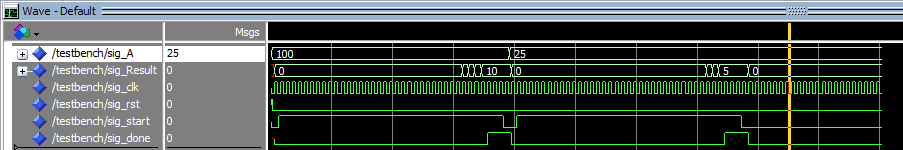
\includegraphics[width=\linewidth]{images/100_25.png}
\caption{Essais $A=100$ puis $A=25$ : résultats 10 et 5.}
\label{fig:10025}
\end{figure}
\begin{figure}[H]
\centering
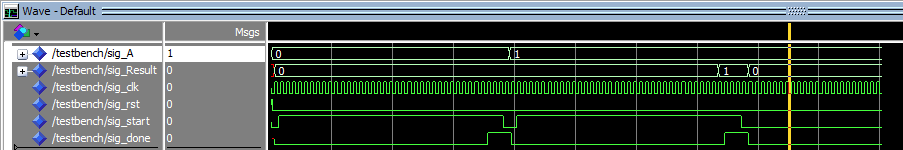
\includegraphics[width=\linewidth]{images/0_1.png}
\caption{Essais $A=0$ puis $A=1$ : résultats 0 et 1.}
\label{fig:01}
\end{figure}
\begin{figure}[H]
\centering
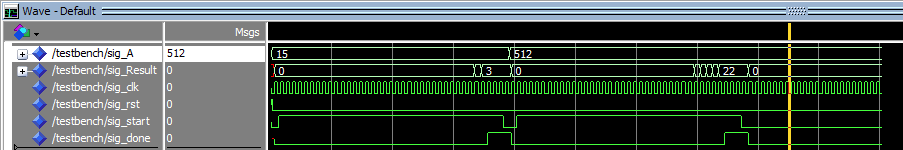
\includegraphics[width=\linewidth]{images/15_512.png}
\caption{Essais $A=15$ puis $A=512$ : résultats entiers 3 et 22.}
\label{fig:15512}
\end{figure}
\begin{figure}[H]
\centering
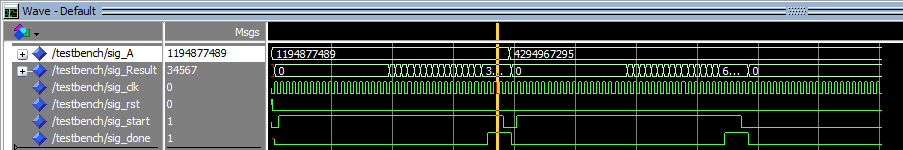
\includegraphics[width=\linewidth]{images/1194877489_4294967295.png}
\caption{Essais sur de grandes valeurs : 34\,567 est lisible au curseur pour le premier calcul ; le résultat du second est tronqué à cette échelle.}
\label{fig:grands}
\end{figure}

\endgroup
\clearpage
\pagestyle{main}
\subsection{Analyse des résultats et limites de validation}
Les figures~\ref{fig:10025} et~\ref{fig:01} confirment les résultats des carrés parfaits et des cas 0 et 1. Pour les valeurs non carrées de la figure~\ref{fig:15512}, le circuit renvoie bien la partie entière : $3^2=9\leq15<16=4^2$ et $22^2=484\leq512<529=23^2$. Pour la première grande valeur, la figure~\ref{fig:grands} affiche 34\,567 lorsque \texttt{done=1}, et $34\,567^2=1\,194\,877\,489$.

\medskip
Les chronogrammes montrent que \texttt{Result} évolue pendant le traitement et reste stable pendant la phase de fin. Les retours à zéro entre deux calculs correspondent à l’exécution de l’état d’attente. La durée de calcul ne dépend pas de l’opérande : même les petites valeurs parcourent les 32 itérations.

\medskip
\textbf{Erreur rencontrée avec un grand opérande.} La figure~\ref{fig:erreur} montre un échec de compilation du testbench sur le littéral décimal \texttt{4294967295}. Le diagnostic indique que cette valeur dépasse \texttt{INTEGER'high}, soit 2\,147\,483\,647 dans cet environnement. Le passage par \texttt{to\_unsigned} ne contourne pas cette limite, car son argument doit déjà être représentable comme un entier naturel. Il s’agit donc d’un problème de construction du stimulus, et non de la largeur de l’entrée $A$, qui possède bien 64 bits.

\begin{figure}[H]
\centering
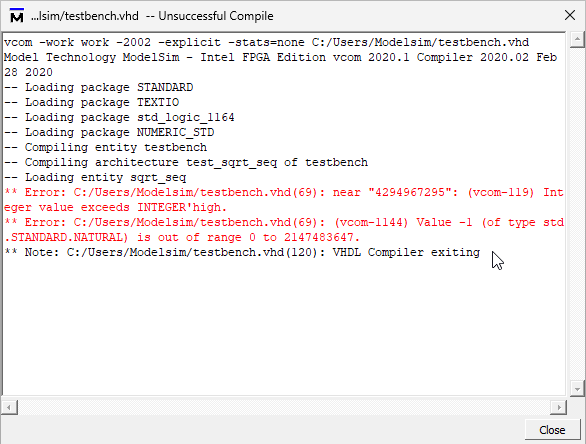
\includegraphics[width=.58\linewidth]{images/error.png}
\caption{Erreur de compilation liée au dépassement du type entier dans le testbench.}
\label{fig:erreur}
\end{figure}

Une solution consiste à affecter directement au bus de 64 bits un littéral hexadécimal sur 64 bits,\\
\texttt{x\textquotedbl00000000FFFFFFFF\textquotedbl}, qui représente 4\,294\,967\,295, sans conversion préalable depuis un entier décimal. La capture de la figure~\ref{fig:grands} montre bien cet opérande sur le bus d’entrée, mais ne documente pas la modification du testbench utilisée pour y parvenir. La valeur attendue est 65\,535, car $65\,535^2\leq 4\,294\,967\,295<65\,536^2$. Une lecture au curseur pendant \texttt{done=1}, ou une assertion, reste nécessaire pour confirmer intégralement ce dernier résultat.

\medskip
\textbf{Portée de cette première validation.} Le testbench présent dans le dossier contient les essais 100 et 25 ; les autres cas sont documentés par les captures de leurs simulations. Il ne comporte pas d’assertions automatiques. Les valeurs testées restent inférieures à $2^{32}$ alors que l’entrée accepte 64 bits : elles ne couvrent donc pas toute la plage $0\leq A\leq2^{64}-1$. Pour compléter la validation, il faudrait notamment tester cette borne supérieure, des valeurs autour de grands carrés parfaits et un reset pendant le calcul.

\medskip
Dans le code actuel, le reset ne réinitialise directement que l’état ; $D$, $Z$, $R$, $i$ et \texttt{done} sont remis à zéro au front qui exécute ensuite l’attente. La sortie peut donc être indéfinie avant ce front au démarrage. Cette particularité doit être prise en compte par l’environnement de commande.

\medskip
\textbf{Conclusion.} L’architecture réalise une itération par cycle dans un seul processus. Les sept résultats entièrement lisibles sont conformes. Le calcul nécessite $n$ cycles, et \texttt{done} est levé après $n+2$ cycles depuis la détection de \texttt{start}. Le dernier grand résultat et la plage complète de 64 bits restent à valider. Les sources associées sont \texttt{sqrt\_seq.vhd} et \texttt{testbench.vhd}.

\end{document}
